

% Algorithm 1 - Self improving loop

% Require : Initial dataset D^0 = {(x_i, y_i) | i \in [N]}, policy model \pi_\theta^0, reward model R, number of self-improving training loop K

% for k ← 1, …, K  do

% Generate synthetic prompts [x_i^1] = Data(\pi_\theta^0, D^0)

% Collect trajectories with MCTS guided by R [y_i^1] = MCTS(\pi_\theta^{k-1}, [x_i^1])

% Construct dataset D^k = {(x_i^k, y_i^k) | i \in [N]}

% Update policy \theta^k = argmin_\theta L(\pi_\theta^k-1, D^k)

% end for

% output \theta^k


% - self-improving problem formulation, transiting to data / search / critic
% - overview
% - data
% - efficient mcts
% -- formulation, s,o,a,r,beta t
% -- mcts
% -- adaptive branching
% -- state fuse
% -- fastrollout
% - Critic Models
% - - value function
% - - process rm
% - - outcome rm

\subsection{Overview}

The architecture of \model{} is depicted in Figure~\ref{fig:framework}, comprising three key components. Firstly, the imagination component is tasked with synthesizing prompts as learning examples. Secondly, an efficient search component, named \emcts{}, is proposed to search high-quality trajectories for optimizing the policy. Lastly, the search process is guided by critics specifically designed to provide reliable signals.

\subsection{Data Synthesizing}

Let $\gD^0 = \{(\vx_i, \vy_i) \mid i \in [N]\}$ denote the initial dataset consisting of $N$ expert-generated prompt-response pairs. The data synthesizing process aims to expand this dataset by generating a set of synthesized prompts $\gD^1 = \{(\vx_i^1,\cdots) \mid i \in [N]\}$. The generation of each synthesized prompt $\vx_i^1$ can be mathematically described as a transformation $g$ applied to one or more examples from $\gD^0$, $\vx_i^1 = g(\vx_{i_1}^0,\cdots,\vx_{i_m}^0, \pi^0)$
% \begin{equation*}
% \vx_i^1 = g(\vx_{i_1}^0,\cdots,\vx_{i_m}^0, \pi^0)
% \end{equation*}
where $\vx_{i_1}^0,\cdots,\vx_{i_m}^0$ are selected examples from $\gD^0$. The transformation function $g$ controls the synthesis process, which can be a learnable function, manually defined heuristic rules, a strong LLM or the policy model itself $\pi^0$ equipped with data synthesis instructions. The data synthesizing process aims to enrich the diversity and complexity presented for the training of the policy model. Among various strategies, such as Self-instruct~\citep{wang2022self}, Evol-instruct~\citep{xu2023wizardlm}, we opt for a method akin to that described in~\cite{yu2023metamath}.

% Challenges and solutions
% 1) Naive MCTS at token level for LLM tasks
% MCTS is a sampling-based search algorithm for policy optimization in decision-making problems. It would iteratively build a search tree, by repeating four phases: selection, expansion, evaluation, and backpropagation. In the selection phase, it would recursively select the children from the root node by Upper Confidence Bound (UCB) bandit ~\cite{auer2002finite}, which is 
% \begin{equation*}
% UCB(i)=w_i+C*\sqrt{2*\ln{\frac{N_i}{n_i}}}
% \end{equation*}
% where $n_i$ and $N_i$ are the visit counts for the node $i$ and its parent respectively, $C$ represents a hyperparameter, and the $w_i$ is the average value of all descendant nodes of $i$. Following selection, the tree undergoes expansion according to the defined policy in the expansion phase. Then in the evaluation phase, the value of the newly expanded node is estimated, by sampling or model-based methods. Finally, in the backpropagation phase, the estimated value is backpropagated to all ancestor nodes of the newly expanded node. 

% To apply MCTS with large language models (LLMs), it is a natural approach ~\cite{liu2023making} to perform search at the token-level, considering each token as an action. However, due to the typically large vocabulary size in LLMs, conducting a deep search becomes very hard as the search space grows exponentially.

% Solution: options
% Following~\cite{option_mcts, de2016monte}, we adapt the term options to represent courses of actions. Typically, an option $o = \langle \gI, \pi, \beta \rangle$, where $\gI \subseteq \gS$ is a set of initial states for the option; $\pi: \gS \times \gA \rightarrow [0,1]$ is a policy to generate actions, which in our case is a LLM; and $\beta: \gS^{+} \rightarrow [0,1]$ is the termination function. Starting from a state $s_t$, we can choose all the options for which $s_t \in \gI$. Once an option is chosen, the policy $\pi$ will generate actions for several steps until the option terminates according to the termination function $\beta$.

% We can then construct the MCTS at the option-level. This means that a new node expansion requires the generation of a complete option, rather than a single token. As a result, the search space is significantly reduced, since the number of options in a trajectory is much fewer than the number of tokens. This allows for a deeper search, more coverage of the search space, and reduces the frequency to request the feedback models, such as the value model. 

% % Policy over options: $\mu: S \times O \rightarrow [0, 1]$ %

% In previous works such as AlphaZero~\cite{silver2018general}, a search tree is built at every step, and the next action is selected based on certain root node statistics, such as visitation frequency. After performing the selected action and receiving the updated state from environment, the tree is built again. This approach is adopted due to the stochasticity of the environment, which requires building the tree based on the most recent actual move. However, in the case of text generation, as the state transition $T$ is deterministic, it is possible to build the tree only once, since all states are accurate. Starting from the initial state, the select-expand-evaluate-backup process is performed several times until a specified condition is met, such as the maximum number of rollouts or terminated nodes. The final answer is then selected from the tree by choosing the optimal trajectory. This offline version of MCTS has also been employed in~\cite{feng2023alphazero}.

% Qs: 
% 2) high efficient MCTS for LLMs
% 3) feedback single for MCTS
% 4) learning

% \subsection{Option-level MCTS}
% % problem defination
% The math problem can be formulated as a Markov Decision Process (MDP): $(S,A,T,R,\gamma)$. The state space $S$ contains information about the math question, as well as answers from previous steps. The action, in the case of segment-level MCTS, is a step of output, thus will be lie in a very large action space $A$. $T$ represent the transition function, which in this case is deterministic. We will only receive reward in the end of each trajectory from reward function $R$, and with the discount factor $\gamma=1$. For each step, we aim to find an optimal action of output that maximize the expected reward $E_{a\sim \pi(a|s)}[\sum_{i=0}^{\infty}\gamma^{i}R(s_{t+1},a_{t+i})]$, where $\pi(a|s)$ is our current policy to solve the problem.

% use Option to defined V/Q


% \subsection{Efficient MCTS}
\subsection{\emcts{}}
\label{sec:mcts}

% \begin{figure}[!t]
    \centering
    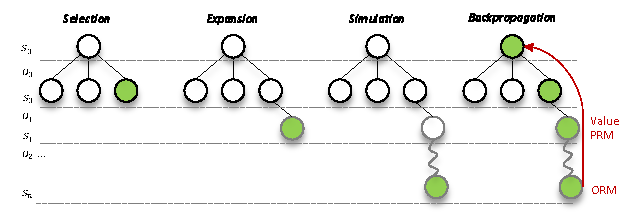
\includegraphics[width=\textwidth]{figures/emcts.pdf}
    \caption{An overview of the four operations of \emcts{}. A node is selected, expanded, simulated with fast rollout policy until a terminal node is reached, then the signals from value function, \prm{} and \orm{} are backpropagated.}
    \label{fig:emcts}
\end{figure}

\subsubsection{Option-level MCTS}

\begin{table}[!htb]
\footnotesize
    \centering
    \setlength{\tabcolsep}{4pt}
    \begin{tabular}{c|c|c}

    \toprule
    \texttt{Search Node} & \texttt{Example} & \texttt{Termination}  \cr
    \midrule
    Token-level & $y_0 \rightarrow y_1 \rightarrow y_2 \rightarrow y_3 \rightarrow y_5 \rightarrow y_6 \rightarrow y_7 \rightarrow y_8$ &  token\cr
    \midrule
    Sentence-level & $y_0 y_1 y_2$ \enterkey{}  $\rightarrow y_4 y_5 y_6$ \enterkey{} $\rightarrow y_7 y_8 y_9 y_{10}$ & new line\cr
    \midrule
    Option-level & $y_0$  $\rightarrow y_1 y_2$ \enterkey{} $\rightarrow y_4 y_5 y_6$ \enterkey{} $y_7 y_8 y_9$ \enterkey{} $\rightarrow y_{10}$& termination function\cr
    \bottomrule
    \end{tabular}
    \vspace{2mm}
    \caption{Comparative illustration of token-level, sentence-level, and option-level MCTS search nodes. $y$ denotes a token sampled from the policy model. The arrow $\rightarrow$ represents the transition from one search node to the subsequent node within the search process.}
    \label{tab:option}
\end{table}


% To apply MCTS to LLMs, it is naturally ~\cite{liu2023making} to performing search at the token-level, considering each token as an action. However, due to the typically large vocabulary size in LLMs, conducting a deep search becomes very challenging as the search space grows exponentially. Some attempts propose sentence-level search where each sentence or step is regarded as an action. While sentence-level search can reduce the complexity of the search space, it might affect the flexibility and performance applying MCTS to LLM as for some tasks subtle variations of several tokens could significantly alter the reward and some tasks might requires more than sentence level search, such as paragraph level search.

% However, the typically large vocabulary of LLMs poses a significant challenge, as conducting a deep search becomes increasingly difficult due to the exponential growth of the search space.

When applying MCTS to LLMs, it is natural to perform token-level search, where each token is considered as an action~\citep{liu2023making}. However, the substantial vocabulary size typical of LLMs presents a significant challenge \ie conducting a deep search in such a vast space becomes increasingly complex as the search space expands exponentially. To mitigate this, some efforts proposed a sentence-level search, treating each sentence or step as a search node~\citep{feng2023alphazero}. While this method reduces the search space, it might compromise the flexibility and effectiveness of applying MCTS to LLMs, which is particularly true for tasks where subtle variations in token can dramatically impact the outcome, or where a more comprehensive search beyond a sentence is necessary.

Inspired by~\cite{option_mcts, de2016monte}, we use the term option as a search node and propose option-level MCTS where each option represents a sequence of tokens, which can range from multiple tokens to several sentences. A comparisons of different levels search is listed in Table~\ref{tab:option}. Mathematically, an option $o = \langle \gI, \pi, \beta \rangle$, where $\gI \subseteq \gS$ is a set of initial states for the option; $\pi: \gS \times \gA \rightarrow [0,1]$ is a policy to generate actions, which in our case is a LLM; and $\beta: \gS^{+} \rightarrow [0,1]$ is the termination function. Starting from a state $s_t$, we can choose all the options for which $s_t \in \gI$. Once an option is chosen, the policy $\pi$ will generate actions for several steps until the option terminates according to the termination function $\beta$. The option-level MCTS consists of stages including selection, expansion, simulation, and backpropagation. The option-level formulation offers more flexibility compared to the sentence-level, as a new line can be treated as a special case of the termination function, as demonstrated in Table \ref{tab:option}. Additional detailed steps of the option-level MCTS can be found in Appendix \ref{app:option_level_mcts}.

% As illustrated in Figure~\ref{fig:emcts}, option-level MCTS consists of the following operations:
% \begin{itemize}[noitemsep,topsep=0pt,parsep=2pt,partopsep=0pt,leftmargin=*]
% \item \textbf{Selection} Starting from the root node, we iteratively select the child node based on Equation \ref{eqs:ucb}.
% \item \textbf{Expansion} Once an expandable leaf node is selected, a new node is generated by starting with the previous state of the parent node as the initial option state. The option is then sampled using the policy $\pi$, and its completion is determined by the termination function $\beta$. 
% \item \textbf{Simulation} The scaled reward of the newly expanded node, as well as some simulated future trajectories are evaluated using the feedback functions, which will be discussed in \S \ref{sec:critic}.
% \item \textbf{Backpropagation} The average value of the newly generated node and all its ancestors is updated using the scaled reward from the evaluation step. Meanwhile, the visit counts for these nodes are also increased by one.
% \end{itemize}

% \begin{itemize}[noitemsep,topsep=0pt,parsep=0pt,partopsep=0pt]
%   \item \paragraph{Selection} Starting from the root node, we iteratively select the child node based on Equation \ref{eqs:ucb}.
% \end{itemize}

%   \item \paragraph{Selection} Starting from the root node, we iteratively select the child node based on Equation \ref{eqs:ucb}.

% \item \paragraph{Expansion} Once an expandable leaf node is selected, a new node is generated by starting with the previous state of the parent node as the initial option state. The option is then sampled using the policy $\pi$, and its completion is determined by the termination function $\beta$. 
%   \item \paragraph{Simulation} The scaled reward of the newly expanded node, as well as some simulated future trajectories are evaluated using the feedback functions, which will be discussed in \S \ref{sec:critic}.
%   \item \paragraph{Backpropagation} The average value of the newly generated node and all its ancestors is updated using the scaled reward from the evaluation step. Meanwhile, the visit counts for these nodes are also increased by one.

% Employing an option to substitute a single token within each node could reduces search space, as the number of options in a trajectory is much smaller than the number of tokens. This facilitates a deeper search, broader coverage of the search space, and minimizes the frequency of requesting feedback from functions such as the value model. Moreover, the option-level offers more flexibility compared to the sentence-level, as a new line can be treated as a special case of the termination function, as demonstrated in Table \ref{tab:option}.

% Policy over options: $\mu: S \times O \rightarrow [0, 1]$ %

% --
% In previous works such as AlphaZero~\cite{silver2018general}, a search tree is built at every step, and the next action is selected based on certain root node statistics, such as visitation frequency. After performing the selected action and receiving the updated state from environment, the tree is built again. This approach is adopted due to the stochasticity of the environment, which requires building the tree based on the most recent actual move. However, in the case of text generation, as the state transition $T$ is deterministic, it is possible to build the tree only once, since all states are accurate. Starting from the initial state, the select-expand-evaluate-backup process is performed several times until a specified condition is met, such as the maximum number of rollouts or terminated nodes. The final answer is then selected from the tree by choosing the optimal trajectory. This offline version of MCTS has also been employed in~\cite{feng2023alphazero}.


% \subsubsection{Importance Weighted Expansion}
% % % Importance weighted expansion
% In previous work related to option/sentence level tree search ~\cite{feng2023alphazero, yao2024tree}, it has been a common practice to assume that each node in the tree has the same predefined width \ie branching factor. This is due to the fact that unlike token-level MCTS with a limited action space, the sample space at the option-level is exceedingly large, with an unlimited number of token combinations. Consequently, it is necessary to set a predefined maximum width and often result in an inefficient search space. For a given node, the error lead by the the branching factor limit can be formulated as
% \begin{equation*}
% E_{\phi} = \mathop{\mathbb{E}}[\min_{i}|v_{\phi}^{\pi}([\vs_t,\vo_t^{new}])-v_{\phi}^{\pi}([\vs_t,\vo_t^{i}])|]
% \end{equation*}
% where $\vo_t^{new}$ is the option of a potential new children that can not be added, $\vo_t^{i}$ represents the current ith children, and $v_{\phi}^{\pi}$ is the value function which will be detailed in \S \ref{sec:critic}. For now we assume that the value of the maximum $m_t$ children nodes are uniform distribution (which is not true but we will cover this in the next part). It is straightforward to show that 
% \begin{equation*}
% E_{\phi} \le \frac{\max_{\vo_t} |v^{\pi}([\vs_t,\vo_t])- v^{\pi}(\vs_t)|}{m_t}.
% \end{equation*}
% While the $E_{\phi}$ is less than some $\epsilon$, we want to use less total number of node for efficiency. And this thus can be formulate as an optimization problem:
% \begin{align*}
% \text{minimize:} & \sum m_t\\
% \text{subject to:} & \frac{\max_{i} |v^{\pi}([\vs_t,\vo_t^{i}])- v^{\pi}(\vs_t)|}{m_t} \le \epsilon
% \end{align*}
% We showed in Appendix that the optimal choice of $m_t$ is proportional to $\frac{1}{m_t}\max_{i} |v^{\pi}([\vs_t,\vo_t^{i}])- v^{\pi}(\vs_t)|$ constant of $1/(\epsilon)$. We name this part as importance $I(\vs_t)$, of the node $\vs_t$.
% \begin{equation*}
% % I(s_t) = \max_{a_t} |Q^{\pi}(s_t,a_t)- E_{a\sim\pi}[Q^{\pi}(s_t,a_t)]|
% I(\vs_t) = \max_{\vo_t} |v^{\pi}([\vs_t,\vo_t])- v^{\pi}(\vs_t)|
% \end{equation*}

% % A more effective and efficient way to determine the branching factor for each node is to dynamically adjust it based on the importance of each node. This approach allows us to allocate a larger child budget to nodes of higher importance, thereby preventing inefficient exploration of these nodes and ensuring that we do not miss promising solutions. Meanwhile, by reducing the number of children for less important nodes, we can perform deeper searches at various levels of the tree, rather than considering all possible options at each node. 

% Similar concept has also be proposed in ~\cite{taylor2014reinforcement, clouse1996integrating}. Intuitively, $I(\vs_t)$ captures the maximum value deviation from the current state. When this value is small, there is no need to explore further on this node, as there will not be a significant difference by rolling out on this node. Conversely, if the value is large, it is worth trying different children. We set the number of children allowed for a node $n(\vs_t)$ to be linear with this importance, using a factor $\alpha$. In practice, to avoid extreme cases of large variance of $I(\vs_t)$ in the early stage, we bound the number of children by depth-dependent constants $c_{\mathtt{min}}(t)$ and $c_{\mathtt{max}}(t)$:
% \begin{equation*}
% n(\vs_t) = \max\left(c_{\mathtt{min}}(t), \min\left(\lfloor \alpha I(\vs_t) \rfloor, c_{\mathtt{max}}(t)\right)\right).
% \end{equation*}

% \subsubsection{Efficient MCTS}
\subsubsection{Importance-Based Adaptive Branching}

In previous works related to option/sentence level tree search ~\citep{feng2023alphazero, yao2024tree}, it was a common practice to assume that each node in the tree has the same predefined width, \textit{i.e.}, branching factor. This assumption was due to the fact that unlike token-level MCTS with a limited action space, the sample space at the option-level is exceedingly large, with an unlimited number of token combinations. As a result, it was necessary to set a predefined maximum width for each node. However, this predefined branching factor is hard to set, as an improper choice can lead to a search tree that is either too shallow or too thin, resulting in an inefficient exploration of the search space.
% As a result, it was necessary to set a predefined maximum width,  which, however, often leads to an inefficient search space.

% \begin{equation*}
% E_{\phi}(t) = \mathop{\mathbb{E}_{\vo_t^{j}\sim \pi(\vs_t)}}[\min_{\vo_{t}^{i}}|v_{\phi}^{\pi}([\vs_t,\vo_t^{j}])-v_{\phi}^{\pi}([\vs_t,\vo_t^{i}])|]
% \end{equation*}
% \begin{equation*}
% I(\vs_t) = \max_{\vo_{t}^{i}} |v_{\phi}^{\pi}([\vs_t,\vo_t^{i}])- v_{\phi}^{\pi}(\vs_t)|
% \end{equation*}
To quantify the error induced by the branching factor limit, we defined the branching error \(E_{\phi}(t)\). For a node \(t\) with a branching factor of \(m_t\), it aims to use the \(m_t\) child options \(\vo_{t}^{i} \sim \gD_{t}^{children}\) (where \(i \in \{1, \ldots, m_t\}\)) to represent all possible options. Consequently, for a legal option \(\vo_{t}^{j} \sim \pi(\vs_t)\) from the option space, we can calculate the minimal value difference between it and the \(m_t\) existing options, which captures the error associated with representing other possible options using the \(m_t\) available options. It can be formulated as 
$E_{\phi}(t) = \mathop{\mathbb{E}_{\vo_t^{j}\sim \pi(\vs_t)}}[\min_{\vo_{t}^{i}}|v_{\phi}^{\pi}([\vs_t,\vo_t^{j}])-v_{\phi}^{\pi}([\vs_t,\vo_t^{i}])|]$, where $v_{\phi}^{\pi}$ is the value function which will be detailed in \S \ref{sec:critic}. Here we define the importance of node $\vs_t$ as $I(\vs_t) = \max_{\vo_{t}^{i}} |v_{\phi}^{\pi}([\vs_t,\vo_t^{i}])- v_{\phi}^{\pi}(\vs_t)|.$ For simplicity, we assume that the value of the children nodes are uniformly distributed (a detailed analysis of the Gaussian distribution can be found in Appendix \ref{app:node_importance_gaussian}). Under this assumption, we show in Appendix \ref{app:node_importance_uniform} that $E_{\phi}(t) \le \frac{I(\vs_t)}{m_t-1}.$
% \begin{equation*}
% E_{\phi}(t) = \frac{I(\vs_t)}{m_t-1}.
% \end{equation*}
While $E_{\phi}$ is less than some $\epsilon$, we aim to use a smaller total number of nodes for efficiency. 
% This can be formulated as an optimization problem:
% \begin{align*}
% \text{minimize:} & \sum m_t\\
% \text{subject to:} & \frac{I(\vs_t)}{m_t} \le \epsilon
% \end{align*}
\newtheorem{theorem}{Theorem}[section]
\begin{theorem}\label{thm:optimal_branching_factor}
The optimal branching factor $m_t$ in a tree search is set such that $m_t - 1$ is proportional to the node importance $I(\vs_t)$, under the condition $\frac{I(\vs_t)}{m_t-1} \le \epsilon$. \normalfont{Refer to Appendix \ref{app:node_importance_uniform} for the detailed proof.}
\end{theorem}
% \begin{proof}
% See Appendix \ref{app:node_importance_uniform}.
% \end{proof}

A similar concept has also been proposed in ~\cite{taylor2014reinforcement, clouse1996integrating}. Intuitively, $I(\vs_t)$ captures the maximum value deviation from the current state. When this value is small, there is no need to explore further on this node, as there will not be a significant difference by rolling out on this node. Conversely, if the value is large, it is worth trying different children. We set the number of children allowed for a node $n(\vs_t)$ (after extracting $1$) to be linear with this importance, using a factor $\alpha$. In practice, to avoid extreme cases of large variance of $I(\vs_t)$ in the early stage, we bound the number of children by depth-dependent constants $c_{\mathtt{min}}(t)$ and $c_{\mathtt{max}}(t)$, $n(\vs_t) = \max\left(c_{\mathtt{min}}(t), \min\left(\lfloor \alpha I(\vs_t) \rfloor+1, c_{\mathtt{max}}(t)\right)\right).$
% \begin{equation*}
% n(\vs_t) = \max\left(c_{\mathtt{min}}(t), \min\left(\lfloor \alpha I(\vs_t) \rfloor+1, c_{\mathtt{max}}(t)\right)\right).
% \end{equation*}

\subsubsection{State Merge}

% With $n(\vs_t)$ determined, another issue is that options under the same node are very similar, leading to many unnecessary sub-trees. Intuitively, we want the distribution of their values to be spread out. As shown in Appendix \ref{app:node_merge}, given a set of values that are evenly distributed, the worst-case error induced by the branching factor limit is minimized.

% Since we cannot directly control the $\vo_t \sim \pi(\vs_t)$, one strategy to make the value distribution of child nodes more evenly spread is to utilize the concept of move groups ~\cite{van2012revisiting}. By merging similar nodes into the same group, we can potentially influence the minimal value gaps between children. This merging allows us to increase the diversity among groups, thereby covering a larger problem space with limited search rollouts and making the search process more efficient.

% Here, we adapt the definition of node predicate $p_{vM}$ from ~\cite{abel2018state} and ~\cite{fu2024accelerating} to represent whether two nodes are extremely similar. In practice, each time we generate a new option from the policy, we use heuristic functions as $p_{vM}$ to check its similarity with all existing groups. The heuristic function can either be a faster rule-based measurement (e.g., edit distance) or a model-based method (e.g., prompting a language model). Based on this, we decide whether to merge this option with a previous one or create a new group. 

With $n(\vs_t)$ determined, another issue is that options under the same node may be very similar, leading to many unnecessary sub-trees. Since we cannot directly control the $\vo_t \sim \pi(\vs_t)$, one strategy to mitigate this issue is to utilize the concept of move groups, as discussed in ~\cite{van2012revisiting}. By merging similar nodes into the same group, we can increase the diversity among groups, thereby covering a larger problem space with limited search rollouts and making the search process more efficient.

Here, we adapt the definition of node predicate $p_{vM}$ from ~\cite{abel2018state} and ~\cite{fu2024accelerating} to represent whether two nodes are extremely similar. In practice, each time we generate a new option from the policy, we use heuristic functions as $p_{vM}$ to check its similarity with all existing groups. The heuristic function can either be a faster rule-based measurement (e.g., edit distance) or a model-based method (e.g., prompting a language model). Based on this, we decide whether to merge this option with a previous one or create a new group. 

% Another explanation, as shown in Appendix \ref{app:node_merge}, is that given a set of values that are evenly distributed, the worst-case error induced by the branching factor limit is minimized. Intuitively, the state merge can also help make the value distribution of child nodes more evenly spread (although not absolutely, as different states may also have similar values).

\subsubsection{Fast Rollout with Specialized LM}

The simulation operation which employs a rollout policy to project future trajectories from a given state, is crucial for an effective MCTS. This process significantly improves the efficiency of exploration and exploitation, and enhances the accuracy of reward estimation\footnote{Typically, the closer the simulation is to the termination state, the more accurate the reward estimation becomes.}. Estimations made at the end of trajectories tend to have lower bias but higher variance; thus, simulating multiple possible trajectories yields low-bias, low-variance estimates, enabling a more informed and effective search process. Ideally, $\pi_\theta$ would serve as the rollout policy, yet its computational demands render it impractical for the rapid simulations required by MCTS. To address this challenge, we propose the use of a smaller, specialized LM as the fast rollout policy $\pi^{\mathtt{fast}}$. Given a state $\vs_t$, the fast rollout policy $\pi^{\mathtt{fast}}$ efficiently continues generation until it reaches a termination condition, denoted as $\pi^{\mathtt{fast}}(\vs_t)$.

\subsection{Critic}
\label{sec:critic}
% It is crucial for searching algorithms to have reliable guidance signals towards achieving the end goal. 
% In \model{}, we design three types of critic models to guide the search process, \ie value function $v^\pi$ predicting the future reward, process reward models \texttt{PRM} estimating node quality, and outcome reward model \texttt{ORM} assessing the overall trajectory quality. 

In \model{}, we design three types of critic models to guide the search process.

% \paragraph{Value Function} The value function, denoted as $v^\pi(\vs)$, is the expected return starting from state $\vs_t$ following the policy $\pi$ thereafter. To train a value function $v^\pi_\phi(\vs)$ parameterized by $\phi$ ~\citep{feng2023alphazero}, we use the Monte Carlo (MC) estimate to empirically approximate the expected reward by averaging the rewards observed after many samplings starting from state $s$ and following policy $\pi$. Thus, the MC estimate of $v^\pi_\phi(\vs)$ can be written as $v^\pi_\phi(\vs) \approx \frac{1}{J} \sum_{j=1}^{J} G^{(j)}(\vs)$ where $J$ is the number of trajectory starting from state $\vs$, $G^{(j)}(\vs)$ is the total discounted reward from state $s$ in the $j$-th trajectory. Particularly, given the expert demonstration dataset $\gD = \{(\vx_i, \vy_i)\}$, for each prompt $\vx_i$, we generate trajectories $\vtau_i^j = \{\vx_i, \vo_{i1}^j, \vo_{i2}^j, \cdots, \vo_{iT}^j \}$ by following policy $\pi$. A reward $r_i^j$ is assigned to indicate whether $\vtau_i^j$ aligns with $\vy_i$, \eg rewarding trajectories that contains correct answers in mathematical tasks or closely follows the instruction as the ground-truth. We then construct a dataset $\gD_{\mathtt{value}} = \{ (\vs_{it}, v_{it}) | i\in[N], t\in[T]\}$ in which $\vs_{it} = [\vx_i\cdot\vo_{<it}]$ and $v_{it} = \frac{1}{J} \sum_{j=1}^{J} r^j_{iT}$. The value function $v_\phi^\pi$ is optimized by minimizing mean squared error $\gL_\phi = - \sE_{(\vs, v)\sim \gD_{\mathtt{value}}} (v_\phi^\pi(\vs) - v)^2$.
% % \begin{equation*}
% % \gL_\phi = - \sE_{(\vs, v)\sim \gD_{\mathtt{value}}} (v_\phi^\pi(\vs) - v)^2
% % \end{equation*}
% We opt to initialize $v_\phi^\pi$ using the parameters from policy $\pi_\theta$, incorporating an MLP layer on top of it to output a scalar on each token. The scalar prediction at the last token of each state is used as the value.
% %, which can be further written as $G_t^{(i)}(s) = \sum_{k=0}^{\infty} \gamma^k R_{t+k+1}^{(i)}$ in which $R_{t+k+1}^{(i)}$ represents the reward received at time $t+k+1$ in the $i$-th trajectory, and $\gamma$ is the discount factor, with $0 \leq \gamma \leq 1$. We create the 

\paragraph{Value Function} The value function, denoted as $v^\pi(\vs)$, represents the expected return starting from state $\vs$ and following policy $\pi$ thereafter, given by $v^\pi(\vs) = \mathop{\mathbb{E}}_{\tau \sim \pi}[R(\tau)|s_0 = \vs]$ where $R(\tau)$ represents the discounted return of trajectory $\tau$. To train a parameterized value function $v^\pi_\phi(\vs)$, given the prompts $\gD = \{(\vx_i, \cdots) \mid i \in [N]\}$, for each prompt $\vx_i$, we generate multiple trajectories $\vtau_i^j = \{\vx_i, \vo_{i1}^j, \vo_{i2}^j, \cdots, \vo_{iT}^j \}$ by following policy $\pi$ for $J$ times. A final reward $r_i^j$ is assigned to indicate whether $\vtau_i^j$ aligns with $\vy_i$—for example, rewarding trajectories that contain correct answers in mathematical tasks or closely follow instructions as ground truth. We then construct a dataset $\gD_{\mathtt{value}} = \{ (\vs^j_{it}, v^j_{it}) \mid i \in [N], t \in [T], j \in [J] \}$ where $\vs^j_{it} = [\vx_i \cdot \vo^j_{<it}]$ and $v^j_{it} = r^j_i$. The value function $v_\phi^\pi$ is optimized by minimizing the mean squared error: $\gL_\phi = - \sE_{(\vs, v) \sim \gD_{\mathtt{value}}} (v_\phi^\pi(\vs) - v)^2$. Similar to ~\citep{feng2023alphazero}, $v_\phi^\pi$ is a LLM with an MLP layer on top to output a scalar on each token, using the scalar prediction at the last token of each state as the value.

% \begin{equation*}
% \gL_\phi = - \sE_{(\vs, v) \sim \gD_{\mathtt{value}}} (v_\phi^\pi(\vs) - v)^2
% \end{equation*}

\paragraph{PRM} The value function often struggles with credit assignment problem~\citep{sutton1984temporal} and its learning could be inefficient due to delayed and sparse rewards~\citep{sutton2018reinforcement}. Therefore, we propose to incorporate \prm{} that introduces process supervision~\citep{lightman2023let} for direct option assessment. \prm{} generates intrinsic rewards~\citep{chentanez2004intrinsically} to encourage explorations of advantageous options, effectively mitigating issues of reward sparsity by providing immediate, action-specific rewards. Given a state $\vs_t$ and an option $\vo_t$ at time $t$, the \prm{} aims to predict the immediate reward $r_t^{\texttt{PRM}}$ that results from taking option $\vo_t$ in state $\vs_t$. Formally, the \prm{} is a function $R(\vs_t, \vo_t) \rightarrow r^{\mathtt{PRM}}_t$. While \prm{} ideally requires quality labels for each state ~\citep{uesato2022solving}, due to the high cost and time involved in obtaining these, MC estimation with prefix sampling~\citep{wang2023math} is used as a proxy, which aligns with the objective of the value function. Instead of adding a MLP layer on top of the policy model for outputting a scalar reward~\citep{ouyang2022training}, we formulate \prm{} as a text generation task to best leverage LLM's intrinsic knowledge for assessing the quality of an option. We adapt the dataset constructed for the value function as $\gD_{\mathtt{PRM}} = \{ (\vs_{it}, \vo_t, r_t^{\mathtt{PRM}} ) | i\in[N], t\in[T]\}$ where $r_t^{\mathtt{PRM}}$ is the textual description of the reward, \eg an option can be regarded as good if $v_{it}$ is larger than certain threshold. To train \prm{},  we initialize it from the policy model $\pi$ and use the following prompt templates and typical language model loss. The prompt template is shown in Appendix \ref{app:prompt}.

% \begin{tcolorbox}[label=prm_prompt]
% \#\#\#[A detailed rubric that specifies how to evaluate a step of a task]\textbackslash n\textbackslash n\#\#\# State\textbackslash n\{\texttt{state}\}\textbackslash n\textbackslash n\#\#\#Action\textbackslash n\{\texttt{option}\}\textbackslash n\textbackslash n\#\#\#Assessment\textbackslash n\{\texttt{textual reward}\}
% \end{tcolorbox}

\paragraph{ORM} In additional to the value function and \prm{}, \orm{} is also used to guide MCTS. \orm{} is designed to evaluate options sequences in their entirety, assessing the extent to which the complete trajectory aligns with the desired end goal~\citep{uesato2022solving,lightman2023let,wang2023math,feng2023alphazero}. The outcome evaluation complements value function and \prm{} by offering a comprehensive assessment of trajectories. Crucially, \orm{} plays a vital role in the simulation stage of MCTS by providing more accurate signals on the terminal state, which in turn facilitates a more balance between exploration and exploitation strategies. \orm{} is formulated as a text generation task, similar to \prm{}. We leverage the same dataset for the value function training and construct $\gD_{\mathtt{ORM}} = \{ (\vx_i, \vo_{1:T}^i, r_i^{\mathtt{ORM}}) | i\in[N]\}$, where each instance includes a initial state or prompt $\vx_i$, a sequence of actions or options $\vo_{1:T}^i$ taken from that state, and a textual reward $r_i^{\mathtt{ORM}}$ indicating the sequence's success or quality. Similarly, \orm{} is initialized from the policy model $\pi$ and the following prompt templates and language model loss are used for training. The prompt template is shown in Appendix \ref{app:prompt}. \\
% \begin{tcolorbox}
% \#\#\#[A detailed rubric that specifies how to evaluate a complete trajectory of a task]\textbackslash n\textbackslash n\#\#\# Prompt\textbackslash n\{\texttt{prompt}\}\textbackslash n\textbackslash n\#\#\#Trajectory\textbackslash n\{\texttt{trajectory}\}\textbackslash n\textbackslash n\#\#\#Assessment\textbackslash n\{\texttt{textual reward}\}
% \end{tcolorbox}

% provide precision feedback on exploirtation

% \begin{equation*}
% s(\vs) = \beta_{\text{value}} \cdot v_\phi^\pi(\vs) + \beta_{\text{PRM}} \cdot \prm{}(\vs) + \beta_{\text{ORM}} \cdot \mathbb{E}_{\tau \sim \pi^{\mathtt{fast}}(\vs)} [\orm{}(\tau)]
% \end{equation*}

The final score evaluation of a state $\vs$ is a weighted sum of the value function, \prm{}, and \orm{}: $s(\vs) = \beta_{\text{value}} \cdot v_\phi^\pi(\vs) + \beta_{\text{PRM}} \cdot \prm{}(\vs) + \beta_{\text{ORM}} \cdot \mathbb{E}_{\tau \sim \pi^{\mathtt{fast}}(\vs)} [\orm{}(\tau)]$, where $\tau \sim \pi^{\mathtt{fast}}(\vs)$ represents trajectories starting from $\vs$ under $\pi^{\mathtt{fast}}$, and $\beta_{\text{value}}$, $\beta_{\text{PRM}}$, $\beta_{\text{ORM}}$ are hyperparameters. In practice, we found that the value function model has better precision and calibration, while \prm{} has superior recall (Appendix \ref{app:critic_performance}). Although \orm{} with fast rollouts provides low-bias, low-variance estimates, it still inherits some bias from $\pi^{\mathtt{fast}}$. Thus, combining these critics yields a stronger evaluation signal.

\subsection{Policy Self-Improvement}
\label{sec:self_improve}

% We have discussed how \emcts{} can guide policy to find trajectories of higher quality and. In this subsection, we discuss how to leverage these trajectories to further improve the policy. It is an iterative process with each iteration containing two main steps: \emph{data generation} and \emph{policy finetuning}.
The policy improvement an iterative process with each iteration containing two main steps: \emph{data generation} and \emph{policy finetuning}.
\paragraph{Data generation} In this step, we assume to have the current policy $\pi_{\theta_k}$ and synthetic prompts $\gD_k=\{\vx^k_1,\dots\}$ at the $k$-th round, where each $\vx^k_1$ represents a question.
We obtain the corresponding training data $\gD_k$ for policy $\pi_{\theta_k}$ by firstly performing \emcts{} on $\gD_k$ (\S \ref{sec:mcts}) and then sampling a trajectory $\vy^k_i$ from the corresponding tree for each question $\vx^k_i$.
% There are several ways to select a trajectory from a MCTS forest, such as taking a greedy path based on the critic score ($w_i$ in Eq. \ref{eqs:ucb}).
Here we choose the trajectory that yield the highest critic score on the leaf node for each input question.
Next, we filter out instances where the corresponding trajectory is substandard forming $\gD_k = \{(\vx^k_i, \vy^k_i)~|~f(\vx^k_i, \vy^k_i)>\gamma\}$
% \begin{equation*}
%  \gD_k = \{(\vx^k_i, \vy^k_i)~|~f(\vx^k_i, \vy^k_i)>\gamma\}
% \end{equation*}
where $f$ represents a function for quality scoring, and $\gamma$ indicates a threshold.
There can be several ways to implement the function, and here we simply use the \orm{} (\S \ref{sec:critic}).

% In this step, we assume to have the current policy $\pi_{\theta_k}$, value network $v^{\pi}$, \orm{} and synthetic prompts $\gD=\{\vx^k_1,\dots\}$, where each $\vx^k_1$ represents a question.
% We obtain the corresponding training data $\gD_k$ for policy $\pi_{\theta_k}$ by first performing MCTS on $D$ (\S \ref{sec:mcts}) and then sampling a trajectory $\vy^k_i$ from the corresponding MCTS forest for each question $\vx^k_i$.
% There are several ways to select a trajectory from a MCTS forest, such as taking a greedy path based on the critic score ($w_i$ in Eq. \ref{eq:mcts}).
% Here we choose the trajectory that yield the highest critic score on the leaf node for each input question.
% As the next step, we filter out instances where the corresponding trajectory is not in high quality:


% consider whether the the final answer of $y^i$ correct (equals to $a^i$).

\paragraph{Policy finetuning}
% With the obtained training data $\gD_k$, we organize the data into the following prompt templates $P_{SI}$:
With the obtained training data $\gD_k$, we organize the data into the prompt templates shown in Appendix \ref{app:prompt}. Then the policy $\pi_{\theta_k}$ is finetuned using target-loss: $\mathcal{L}_{\theta_k} = \mathbb{E}_{(\vx^k_i, \vy^k_i) \sim \gD_k} \big[\log \pi_{\theta_k}(\vy^k_i|\vx^k_i) \big]$, resulting in an updated policy $\pi_{\theta_{k+1}}$. We leave other training methods, such as DPO \citep{rafailov2023direct} or PPO \citep{schulman2017proximal} in future work.
% \begin{equation*}
%  \mathcal{L}_{\theta_k} = \mathbb{E}_{(\vx^k_i, \vy^k_i) \sim \gD_k} \big[\log \pi_{\theta_k}(\vy^k_i|\vx^k_i) \big]
% \end{equation*}
% This results in an updated policy $\pi_{\theta_{k+1}}$.
% We leave other training methods, such as DPO \citep{rafailov2023direct} or PPO \citep{schulman2017proximal} in future work.
% With the new policy, the value network and ORM is then updated as described in \S \ref{}.